%%%%%%%%%%%%%%%%%%%%%%%%%%%%%%%%%%%%%%%%%
% Simple Sectioned Essay Template
% LaTeX Template
%
% This template has been downloaded from:
% http://www.latextemplates.com
%
% Note:
% The \lipsum[#] commands throughout this template generate dummy text
% to fill the template out. These commands should all be removed when 
% writing essay content.
%
%%%%%%%%%%%%%%%%%%%%%%%%%%%%%%%%%%%%%%%%%

%----------------------------------------------------------------------------------------
%	PACKAGES AND OTHER DOCUMENT CONFIGURATIONS
%----------------------------------------------------------------------------------------

\documentclass[12pt]{article} % Default font size is 12pt, it can be changed here

\usepackage{natbib}
\bibliographystyle{plainnat}
\usepackage{url}


\usepackage[portuges]{babel}
\usepackage[utf8]{inputenc} % Acentuação
\usepackage{indentfirst}
\setlength{\parskip}{\baselineskip} % Space between paragraphs

\usepackage{geometry} % Required to change the page size to A4
\geometry{a4paper} % Set the page size to be A4 as opposed to the default US Letter

\usepackage{graphicx} % Required for including pictures

\usepackage{float} % Allows putting an [H] in \begin{figure} to specify the exact location of the figure
\usepackage{wrapfig} % Allows in-line images such as the example fish picture

\usepackage{lipsum} % Used for inserting dummy 'Lorem ipsum' text into the template

\linespread{1.2} % Line spacing

%\setlength\parindent{0pt} % Uncomment to remove all indentation from paragraphs

\graphicspath{{./pictures/}} % Specifies the directory where pictures are stored

\begin{document}

%----------------------------------------------------------------------------------------
%	TITLE PAGE
%----------------------------------------------------------------------------------------

\begin{titlepage}

  \newcommand{\HRule}{\rule{\linewidth}{0.5mm}} % Defines a new command for the horizontal lines, change thickness here

  \center % Center everything on the page

  
\includegraphics{logo}\\[1cm] % Include a department/university logo - this will require the graphicx package

  \textsc{\LARGE Universidade do Minho}\\[1.5cm] % Name of your university/college
  \textsc{\Large Sistemas Distribuídos}\\[0.5cm] % Major heading such as course name
  %\textsc{\large Minor Heading}\\[0.5cm] % Minor heading such as course title

  \HRule \\[0.4cm]
  { \huge \bfseries Projecto Integrado}\\[0.1cm] % Title of your document
  { \small Um sistema de troca de mensagens com Ruby e Websockets }
  \HRule \\[0.8cm]

  \begin{flushleft}
    Gabriel Poça, PG22804 \\
    Rafael Remondes, PG99999
  \end{flushleft}


  {\large \today}\\[3cm] % Date, change the \today to a set date if you want to be precise

  \begin{abstract}
    Procura explorar as potencialidades da linguagem Ruby de modo a oferecer
    a clientes web um plataforma de troca de mensagens.
  \end{abstract}


  \vfill % Fill the rest of the page with whitespace

\end{titlepage}

%----------------------------------------------------------------------------------------
%	TABLE OF CONTENTS
%----------------------------------------------------------------------------------------

\tableofcontents % Include a table of contents

\newpage % Begins the essay on a new page instead of on the same page as the table of contents 

%----------------------------------------------------------------------------------------
%	INTRODUCTION
%----------------------------------------------------------------------------------------


\section{Introdução}

Este documento serve o propósito de documentar o estudo e desenvolvimento levado a cabo no projecto integrado da unidade curricular de sistemas distribuídos.

As próximas secções desta introdução introduzem conceitos e tecnologias utilizadas com o objectivo de suportar as análises posteriores no relatório.





\section{Introdução Teórica}

Esta secção serve de introdução teórica aos conceitos utilizados ao longo do relatório. O objectivo é relembrar o fundamental e establecer a terminologia a utilizar no desenvolvimento do relatório.

% ---------------------- Message Oriented Middleware

\subsection{Message oriented middleware (MOM)} 

Entende-se por \textit{message oriented middleware} (MOM) como um método de comunicação entre componentes de sistemas distribuídos.

\begin{description}
  \item[Assincrono] \hfill \\
  	Permite que um cliente não bloqueie enquanto espera por resposta.
  \item[Second]
  \item[Third] The third etc \ldots
\end{description}

No contexto deste relatório entede-se por MOM como uma camada de comunicação que permite a várias aplicações comunicar ignorando as especificidades de cada uma.

% ---------------------- Websockets

\subsection{Introdução a websockets}

A conceção inicial da web considerou apenas a comunicação cliente-servidor num sentido apenas. Actualmente o HTML5 procura corrigir esta entrave, contudo ainda muitos projectos utilizam \textit{long-polling} para simular a comunicação cliente-servidor.

Actualmente os browsers são actualizados regularmente e suportam a API de comunicação do HTML5.

\subsubsection{\textit{Long pulling}}

\begin{figure}[H]
\centering
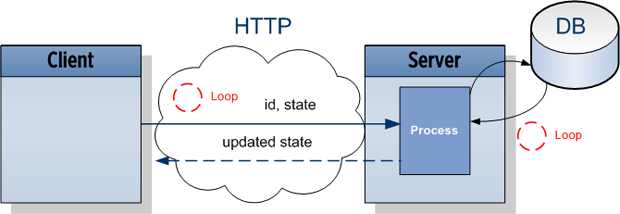
\includegraphics[width=0.9\textwidth]{longpolling-architecture.png}
\caption{Esquema de \textit{long pulling}}
\label{fig:long_pulling}
\end{figure}

Um cliente (browser) envia por HTTP um pedido para o servidor com o identificador do utilizador (por exemplo) e do estado actual. No servidor é criado um processo que repetidamente verifica na base de dados se existe um estado novo. Quando existe um novo estado o cliente recebe e envia um novo pedido ao servidor.

\subsubsection{\textit{Server-Sent Events}}

\begin{figure}[H]
\centering
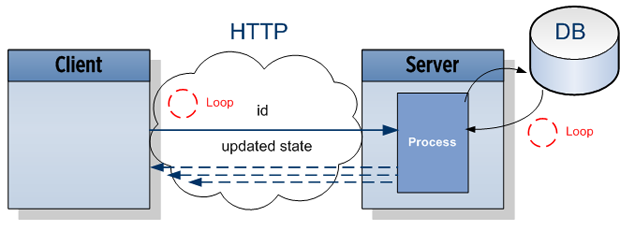
\includegraphics[width=0.9\textwidth]{sse-architecture.png}
\caption{Esquema de \textit{server-sent events}}
\label{fig:sse-architecture}
\end{figure}

Um cliente (browser) faz um pedido ao servidor. O servidor responde com o último estado na base de dados. O cliente recebe a resposta e em três segundos (por exemplo) envia um novo pedido.

\subsubsection{Websockets}

\begin{figure}[H]
\centering
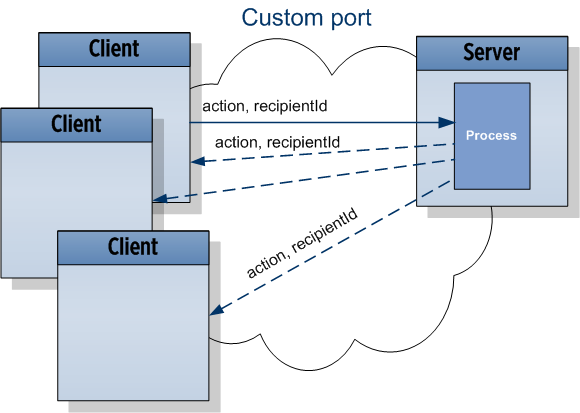
\includegraphics[width=0.9\textwidth]{websocket-architecture.png}
\caption{Esquema de \textit{websockets}}
\label{fig:websockets-architecture}
\end{figure}

Um cliente notifica o servidor de websockets de um evento. O servidor imediamente notifica todos os clientes ativos do evento. Este processo pode envolver filtros e subscrição de eventos.


\section{Ferramentas}

As próximas secções introduzem ferramentas utilizadas no projecto, desde bibliotecas ruby e javascript a base de dados.

\subsection{Ruby}

Ruby é uma linguagem de programação intrepertada com suporte para diferentes paradigmas (funcional, orientado a objectos e imperativo). Desde o lançamento em 1995 Ruby tem crescido em comunidade e potencial. O seu criador, Yukihiro Matsumoto, pretendia uma linguagem que qualquer programador pudesse aperciar:

``Ruby is simple in appearance, but is very complex inside, just like our human body.'' \cite{matz}

Ruby encontra-se actualmente na versão 2.0.0-p195 no entanto o projecto foi desenvolvido na versão \textbf{2.0.0p0}.

\subsubsection{\textit{Global Interpreter Lock}}

Existem diversos intrepertadores para Ruby sendo os mais importantes \textbf{Matz's Ruby Interpreter (MRI)}, em homenagem ao criador, e \textbf{JRuby}, implementado no topo da Java Virtual Machine. 
A diferença mais relevante entre ambos para este projecto é o \textit{Global Interpreter Lock} (GIL) que existe no MRI. O GIL é uma camada responsável por proteger o intrepertador contra código \textit{non thread-safe}.

A figura~\ref{fig:ruby-gil} apresenta uma comparação entre três versões do Ruby. Na versão 1.8 o intrepertador Ruby possuí apenas uma thread do sistema para execussão. Já na versão 1.9, e também na versão 2 ainda que não seja visível na imagem, várias threads do sistema são alocadas ao intrepertador, o que parece prometer paralelismo de execussão. No entanto em ambos os casos existe a camada do GIL que protegendo contra a execussão de código \textit{non thread-safe} permite que apenas uma thread seja executada de cada vez pelo processador, ou seja, ambas as versões do Ruby correm num core do CPU apenas.
Por outro lado a implementação em JRuby não contém a camada GIL o que abre as portas ao paralelismo das aplicações em Ruby.

\begin{figure}[H]
\centering
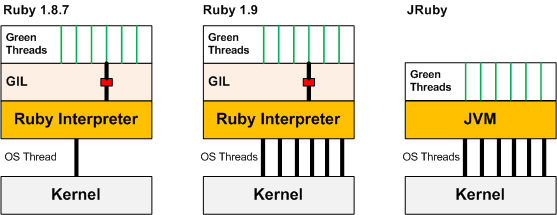
\includegraphics[width=0.9\textwidth]{xruby_gil.png}
\caption{\textit{Global Interpreter Lock}}
\label{fig:ruby-gil}
\end{figure}

Parecendo um cenário desvantajoso para o MRI é de notar que existem soluções para contornar este problema. Se se pensar em processos em vez de threads por procurar-se outros meios de repartir trabalho. Decompondo a aplicação e adicionando meios de comunicação entre processos (Starling, RabbitMQ, outros) consegue-se que multiplos processos da mesma aplicação executem concurrentemente.

\subsubsection{RubyGems}

A aplicação do servidor, em Ruby, encontra-se no formato RubyGem, geralmente denominado por gem. O software RubyGem permite que facilmente se descarregue, instale e manipule gems num sistema.\cite{rubygems} O que se pretende com esta preocupação é permitir que a aplicação possa facilmente ser distribuída e desse modo contribuir para a comunidade Ruby.

Em modo muito básico uma gem é composta pelo seguinte:

\begin{description}
\item[Gemspec] Ficheiro que identifica as dependência da gem. No caso deste projecto o nome do ficheiro é \textit{eventmachinemom.gemspec}.
\item[Código da aplicação] Código a executar pela aplicação, encontra-se na pasta \textit{lib}.
\item[Testes] Testes da aplicação. No caso deste projecto os testes são \textbf{RSpec} e encontram-se na pasta \textit{spec}.
\item[Excutáveis] Ficheiros executáveis que são instalados no sistema que podem ser invocados pelo utilizador ou outro software. Encontram-se na pasta \textit{bin}.
\end{description}

\subsubsection{EventMachine}

EventMachine é uma biblioteca para Ruby que implementa \textit{event-drive I/O}. Ruby não foi concebido para executar concorrentemente nem para suportar programação por eventos.




A biblioteca é utilizada em servidores de eventos; servir clientes assincronos por diferentes protocolos; proxys. \textbf{EventMachine Websockets}

\subsubsection{ActiveRecord}
Esta ferramenta é já parte do cliente.
Active Record é um biblioteca Ruby que establece uma ligação entre classes e tabelas de bases de dados relacionais sem grande configuração. Esta biblioteca uma classe base que quando é extendida establece um mapeamento entre a nova classe e um tabela existente na base de dados. A biblioteca foi desenvolvida inicialmente para a framework Ruby on Rails sendo o base do que se chama models.

É importante referir que o uso desta biblioteca permite que não se escreva SQL de de operações sobre a base de dados à excepção da criação de tabelas sendo esta processo gerado por operações em Ruby.

\subsection{PostgreSQL}

No primeiro esquema conceptual da arquitectura da aplicação planeou-se utilizar SQLite, cada broker teria a sua base de dados e depois haveria sincronização entre todos. 

A primeira abordagem além de complexa não explora o \textbf{controlo de concurrência} que grande parte das base de dados oferece como garantido. Como tal a nova abordagem passa por centralizar a base de dados e todos os servidores trabalham sobre a mesma conseguindo-se sincronização e controlo de concurrência.

\subsection{JQuery}

jQuery é uma biblioteca JavaScript que facilita a manipulação de HTML, eventos, animação, Ajax com uma API transversal aos browsers. Juntamente com a biblioteca JQuery faz-se uso da biblioteca \textbf{The Graceful WebSocket} que permite fornece um sistema de fallback para websockets.



%----------------------------------------------------------------------------------------
%	CONCLUSION
%----------------------------------------------------------------------------------------

\section{Conclusion} 

%----------------------------------------------------------------------------------------
%	BIBLIOGRAPHY
%----------------------------------------------------------------------------------------

%\bibliographystyle{plain}
\begingroup
\raggedright
\bibliography{bibliography.bib}
\endgroup

%----------------------------------------------------------------------------------------

\end{document}
